%%%%%%%%%%%%%%%%%%%%%%%%%%%%%%%%%%%%%%%%%%%%%%%%%%%%%%%%%%%%%%%%%%%%%%%%%%%%%%%%
%2345678901234567890123456789012345678901234567890123456789012345678901234567890
%        1         2         3         4         5         6         7         8

\documentclass[letterpaper, 10 pt, conference]{ieeeconf}  % Comment this line out
                                                          % if you need a4paper
%\documentclass[a4paper, 10pt, conference]{ieeeconf}      % Use this line for a4
                                                          % paper

\IEEEoverridecommandlockouts                              % This command is only
                                                          % needed if you want to
                                                          % use the \thanks command
\overrideIEEEmargins
% See the \addtolength command later in the file to balance the column lengths
% on the last page of the document

\usepackage{graphicx}
\usepackage{multicol}
\usepackage{subfigure}
\usepackage{mathptmx} % use Times fonts if available on your TeX system
\usepackage{setspace}
\usepackage{algorithmicx}
\usepackage{algpseudocode}
% The following packages can be found on http:\\www.ctan.org
%\usepackage{graphics} % for pdf, bitmapped graphics files
%\usepackage{epsfig} % for postscript graphics files
%\usepackage{mathptmx} % assumes new font selection scheme installed
%\usepackage{times} % assumes new font selection scheme installed
%\usepackage{amsmath} % assumes amsmath package installed
%\usepackage{amssymb}  % assumes amsmath package installed

\title{\LARGE \bf
Decentralized Communications for Self-regulated\\ Division of Labour in Robot Society
}

\author{ Md Omar Faruque Sarker and Torbj{\o}rn S. Dahl\\
         %\thanks{This research has been funded by the Engineering and Physical Sciences 				Research Council (EPSRC), UK, grant reference EP/E061915/1.}%
        Robotic Intelligence Lab, Newport Business School\\
		University of Wales, Newport, Allt-yr-yn Campus\\ 
		Allt-yr-yn Avenue, Newport, NP205XR, UK\\
		{\tt\small Mdomarfaruque.Sarker@newport.ac.uk}\\ 
		{\tt\small Torbjorn.Dahl@newport.ac.uk}      
}

%\author{Huibert Kwakernaak and Pradeep Misra% <-this % stops a space
%\thanks{This research has been funded by the Engineering and Physical Sciences Research Council (EPSRC), UK, grant reference EP/E061915/1.}% <-this % stops a space
%%\thanks{H. Kwakernaak is with Faculty of Electrical Engineering, Mathematics and Computer Science,
%%        University of Twente, 7500 AE Enschede, The Netherlands
%%        {\tt\small h.kwakernaak@autsubmit.com}}%
%%\thanks{P. Misra is with the Department of Electrical Engineering, Wright State University,
%%        Dayton, OH 45435, USA
%%        {\tt\small pmisra@cs.wright.edu}}%
%}


\begin{document}


\maketitle
\thispagestyle{empty}
\pagestyle{empty}


%%%%%%%%%%%%%%%%%%%%%%%%%%%%%%%%%%%%%%%%%%%%%%%%%%%%%%%%%%%%%%%%%%%%%%%%%%%%%%%%
\begin{abstract}

Distributed local communication is one of the essential means by which various social insects achieve their self-regulatory division of labour (SRDL). Unlike centralized static communication, this communication mode enables individuals to respond to local changes quickly and it generally produces steady-state convergence of SRDL in social insects. However, realizing this kind of communication in a distributed multi-robot system (MRS) is not as straight forward as a centralized one. From a robot controller's point of view, it is not easy to determine how often or how much dynamic peer-to-peer (P2P) communication is needed to maintain system's convergence of SRDL. To deal with this issue, in this paper, we first present a model for dynamic local communication and its implementation on a MRS with two different communication radii. Then we compare this system with our baseline centralized communication based MRS in terms of convergence of SRDL, communication load, robot task specializations and their motions.  Results from these experiments suggest us that similar or better convergence of SRDL can be obtained by setting a smaller P2P communication radius where a robot locally exchanges signals with a minimum number of its nearby peers. Our experiments used 16 e-puck robots in a 2m X 2m area.
%
\end{abstract}
%
%%%%%%%%%%%%%%%%%%%%%%%%%%%%%%%%%%%%%%%%%%%%%%%%%%%%%%%%%%%%%%%%%%%%%%%%%%%%%%%%
\section{INTRODUCTION}
\label{sec:intro}
Self-regulated division of labour (SRDL) is one of the key research issues in the filed of multi-agent and multi-robot systems (MRS). Inspired from biological and various other social systems, robotic researchers have achieved SRDL in MRS using various forms of communications \cite{Bonabeau+1999 - Labella}. Two basic forms of communications are: 1) direct or explicit communication and 2) indirect or implicit communication. Direct communication is an intentional communicative act of message passing that  aims at one or more particular receiver(s) \cite{Mataric}. It typically exchanges information  through physical signals. In contrast,  indirect communication, sometimes termed as {\em  stigmergic} in biological literature, happens as a form of modifying the environment (e.g., pheromone dropping by ants) \cite{Bonabeau+1999}.  In ordinary sense, this is an observed behaviour and many researchers call it as {\em no communication} \cite{Labella}. In order to avoid ambiguity, by the term {\em communication},  we always refer to direct communication. In this paper, we also confine our discussion on SRDL within the context of direct communication only.\\
In order to pursue a SRDL,  robots can receive information from a centralised source \cite{Krieger} or from their local peers \cite{Agassounon}. In \cite{Sarker}, we reported a steady-state convergence of SRDL in a practical MRS using a centralized information source.  This  centralized communication system  is easy to implement and it simplifies the overall design of  a robot controller. However this system has disadvantage of a single point of failure and it is not scalable. The increased number of robots and tasks cause  inevitable increase in communication load and  transmission delay and as a consequence, the overall system performance degrades.  On the other hand, uncontrolled reception of information from decentralized or local sources is also not  free from drawbacks. If a robot exchanges signals with all other robots (hereafter called as {\em peers}), it might get the global view of the system quickly and can select an optimal  or near optimal task. This can produce a great improvement in overall performance of some types of tasks e.g., in area coverage \cite{Rutishauser}. But this is  also not practical and scalable for a typically large MRS due to the limited communication and computation capabilities of robots and limited available communication bandwidth.\\ 
A potential alternate solution to this problem can be obtained by decreasing the number of message recipient peers on the basis of a local communication radius (CR). This means that robots are allowed to communicate only with those peers who are physically located within a preset distance. When this strategy is used for sharing task information among peers, SRDL can be more robust and efficient. This concept was validated by simulation in \cite{Agassounon}. But they did not give us any insight for choosing the value of CR. In this paper, we have presented a set of experimental results of SRDL in our MRS with two values of CR: 0.5m and 1m. In case of the former one, we call the peers located within CR as {\em nearby peers}. Similarly in case of latter one, we call the peers located within CR as {\em distant peers}. Along with a practical insight for selecting CR value, various other design issues have been tackled in this paper. The recursion-free design of  local communication channels is achieved by a dynamic publish/subscribe model of communication. This has been validated by using a state-of-the-art D-Bus \footnote{http://dbus.freedesktop.org/doc/dbus-specification.html}. inter-process communication technology in Linux.\\
Our contributions from this study are as follows. We present a dynamic publish/subscribe local model of communication that achieves similar or better SRDL than its centralized counterpart. The reduction of robot motion is half in this case and this tells us about the level of impact this local model can make on the energy efficiency of a MRS. The reduction in communication load in local model  is also significant.  Unlike a fixed communication frequency, the dynamic variation in communication frequency produced by by our local model suggests us that local communication model should be preferred to a centralized one when robustness and scalability of SRDL of a MRS is an important issue.

Rest of the paper is organized as follows. Section~\ref{sec:bg} discusses related background works. Section~\ref{sec:model} presents our local communication model that allows us to implement a inter-disciplinary generic model of SRDL as a multi-robot task allocation (MTRA) mechanism. Section~\ref{sec:impl} introduces our implementation of MRTA including the interactions between the hardware, software and communication modules. Section~\ref{sec:expt-design} presents the design of our experiments including specific parameters and observables. Section~\ref{sec:results} discusses our experimental results and section~\ref{sec:conc} draws conclusions.
%
%%%%%%%%%%%%%%%%%%%%%%%%%%%%%%%%%%%%%%%%%%%%%%%%%%%%%%%%%%%%%%%%%%%%%%%%%%%%%%%%
\section{Related Works}
\label{sec:bg}

%%%%%%%%%%%%%%%%%%%%%%%%%%%%%%%%%%%%%%%%%%%%%%%%%%%%%%%%%%%%%%%%%%%%%%%%%%%%%%%%
\section{Modeling}
\label{sec:model}
\subsection{Model for Self-Regulatory DoL}
Our model of self-regulated DoL is based on AFM. It provides us a generic framework for implementing self-regulatory DoL in robots. Here we briefly describe how this model gives our robots self-regulatory DoL behaviours, particularly task-specialization, concurrency, flexibility and robustness.
Let us consider a manufacturing shop floor scenario where N number of mobile robots are required to attend to M number of shop tasks spread over a fixed area A. Let these tasks be represented by a set of small rectangular boxes resembling to manufacturing machines. Let $R_1$, $R_2$ … $R_n$ be the set of all robots and $J_1$, $J_2$ … $J_m$ be the set of all tasks. Each task $j$ has an associated task-urgency $\phi_j$ that indicates its relative importance over time. If a robot attends to a task $j$ in x$^{th}$ time-step, value of $\phi_j$ will decreases by a small amount $\delta_\phi$ in (x+1)$^{th}$ time-step. On the other hand, if a task has not been served by any robot in x$^{th}$ time-step,  $\phi_j$  will increase by another small amount in (x+1)$^{th}$ time-step. In order to complete a shop task $J_1$, a robot $R_1$ needs to reach within a fixed boundary $D_j1$ of $J_1$. If a robot completes a task $j$ we say that it learns about it and this will increase robot's likelihood of selecting that task in next step. We call this variable affinity of a robot to that task as its sensitization $k_j$ . If a robot does not do a task $j$ for some time, we say that it forgets about $j$ and $k_j$ has been decreased.\\
According AFM, all robots will establish attractive fields to all tasks due to the presence of a system-wide continuous flow of information. The strength of these attractive fields called stimulus will vary according to the distances between robots and tasks, task-urgencies and corresponding  sensitizations of robots. This is encoded in Eq. \ref{eqn1}.
%\addtolength{\abovedisplayskip}{-15mm} 
\begin{small}
%\begin{multicols}{2} 
\begin{equation}
S_{j}^{i} = tanh\{\frac{k_{j}^{i}}{d+\delta } \phi _{j}\}
\label{eqn1}
\end{equation}
%\vspace*{0.25cm}
\begin{equation}
P_{j}^{i} = \frac{S_{j}^{i}}{\sum_{j}^{}S_{j}^{i}}
\label{eqn2}
\end{equation}
%\end{multicols}
\end{small}
%\addtolength{\belowdisplayskip}{-1mm} 
%\vspace{2mm}
Eqn \ref{eqn1} says that the stimuli of a robot $i$ to a particular task $j$, $(S_{j}^{i})$ depends on robot's spatial distance $d$ to $j$, level of sensitization to that task ($k_{j}^{i}$) and perceived urgency of that task ($\phi _{j}$). We use a vary small value $\delta$ in \ref{eqn1} to prevent  division by zero. The probability of selecting each task has been determined by a probabilistic method outlined in Eq. \ref{eqn2} . 
AFM suggests concurrency of a self-regulatory system by specifying at least two task options: 1) doing a task and 2) doing no task. In robots, the latter can be   be treated as random walking. So in any time-step a robot will choose from M+1 tasks. Let $T_a$ be the allocated time to accomplish a task. If $R_1$ can enter inside the task boundary within $T_a$ time it waits there until $T_a$ elapsed. Otherwise it will select a different task. 

\section{Our Dynamic P2P Communication Model}
\label{sec:comm}
\subsection{Characteristics}
This model is based on the local P2P communications among robots. Here there is no centralized server to disseminate information but each robot can communicate to its nearby peers within its communication radius, $r_{comm}$. Here by $r_{comm}$, we assume that within this distance robots can exchange communication signals reliably without any significant loss of information or delay. A robot $R_1$ is a nearby peer  of robot $R_2$, if spatial distance between $R_1$ and $R_2$ is less than its $r_{comm}$. As shown in Fig. \ref{fig:lcm}, local communication can also give robots similar task information as in centralized communication mode. It shows that  it is not necessary for each robot to communicate with every other robot to get information on all tasks. Since robots can random walk  and explore the environment we assume that for a reasonably high robot to space density, all task will be known to all robots after an initial exploration period. In order to update the urgency of a task, robots can estimate the number of robots working on a task either by using their sensory perception (e.g., camera)  or by doing local P2P communication. In Fig. ref{fig:lcm} we have shown that robots exchange both TaskInfo and RobotStatus signals to peers.

We characterize our communication model in terms of three fundamental issues: 1) message content ({\em what to communicate}) 2) communication frequency ({\em when to communicate})  and 3) target recipients ({\em with whom to communicate})  \cite{Gerkey}. In a typical MRS, message content can be categorized into two types: 1) state of each individual robot  and 2) target task (goal) information \cite{Balch}. The latter can also be subdivided into two types: 1) an individual robot's target task  information 2) information of all available tasks found in the system. Regarding the first issue, our communication model is open. Robots can communicate with their peers with any kind of message. Our model addresses the last two issues very specifically. Robots  communicate only when they meet their peers within a certain communication radius (CR). Although in case of an environment where robots move relatively faster the peer relationships can also be changed dynamically. But  this can be manipulated by setting  the signal frequency and robot to space density to some reasonably higher value. In terms of target recipients, our model differs from a traditional publish/subscribe communication model by introducing the concept of dynamic subscription. In a traditional model subscription of messages happens prior to the actual message transmission. In that case prior knowledge about the subjects of a system is necessary. But in our model this is not necessary as long as all robots uses a common addressing convention for  naming their incoming  signal channels. In this way, when a robot meets with another robot it can infer the address of this peer robot's target  channel name by using a static rule.  A robot is thus always listening to its own channel for receiving messages from its potential peers or message publishers. On the other side, upon recognizing a peer a robot sends a message to this particular peer aiming at its inferred outgoing channel. So here it neither necessary to create any custom subject namespace nor to hard-code information in each robot controller about the names of their potential peers. Subscription is done automatically based on its  $r_{comm}$.

\subsection{Implementation Algorithm}
%
Let N be the set of robots and a robot $i$ has a channel $L_i$ for reception of signals directed to itself. Let M be the set of  tasks and each task $j$ has an associated information $H_j$. It encodes the necessary properties of tasks, such as their locations, urgencies etc. Each task  $j$ also has a task perception radius $r_{task}$ such that if a robot comes within this radius it can perceive current value of $H_j$.  Let at time step q, robot $i$ has its own task information $G_{i}^{q}$ that contains all or a subset of all task information. Let $r_{comm}$ be the communication range of each robot. 
Let at time step q, $P_{p, q}^{i}$ be a set of peer robots of $i$ that are within $r_{comm}^{i}$. Let $E_{p, q}^{i}$ be its active signal emission channels. Algorithm 1
shows implementation of our proposed P2P dynamic communication.\\    
% 
\textbf{\small Algorithm 1: Locality based Dynamic P2P Communication}
\begin{algorithmic}[1]
\label{alg:p2p-comm}
\State $\textbf{Initialization:}$
	\State $robotid \gets id$
	\State $pose[id] \gets (0, 0, 0)$
	\State $G[id], ~P[id], ~L[id], ~E[~] \gets 0$
\State $\textbf{Loop:}$
	\State $pose[id] \gets (x, y, \theta)$
	% PERCEPTION of TASK
	\If {$pose[id]  \in U(pose[k],~ r_{task}^{k}), (k = 0, 1, …., M-1)$} 
		\State $G[id] \gets G[id] ~\cup ~ H_k$
	\EndIf
	% P2P Interaction, listen signal
	\If {$pose[id]  \in V(pose[k],~ r_{comm}^{k}), (k = 0, 1, …., N-1, k\neq id )$} 
		\State $P[id] \gets P[id] ~ \cup ~ k$
		\State  $h_k \gets W(E[k],~ L[id])$
		\State $G[id] \gets G[id] ~ \cup ~ h_k$
	\EndIf
	% P2P Interaction, emit signal
	\ForAll {$ k \in P[id], (k = 0, 1, …., N-1, k\neq id)$}
		\State $ W(E[id],~L[k]) \gets G[id]$
	\EndFor
\State $\textbf{Loop again}$
\end{algorithmic}

%\addtolength{\floatsep}{-25mm}
\begin{figure}[thpb]
\centering
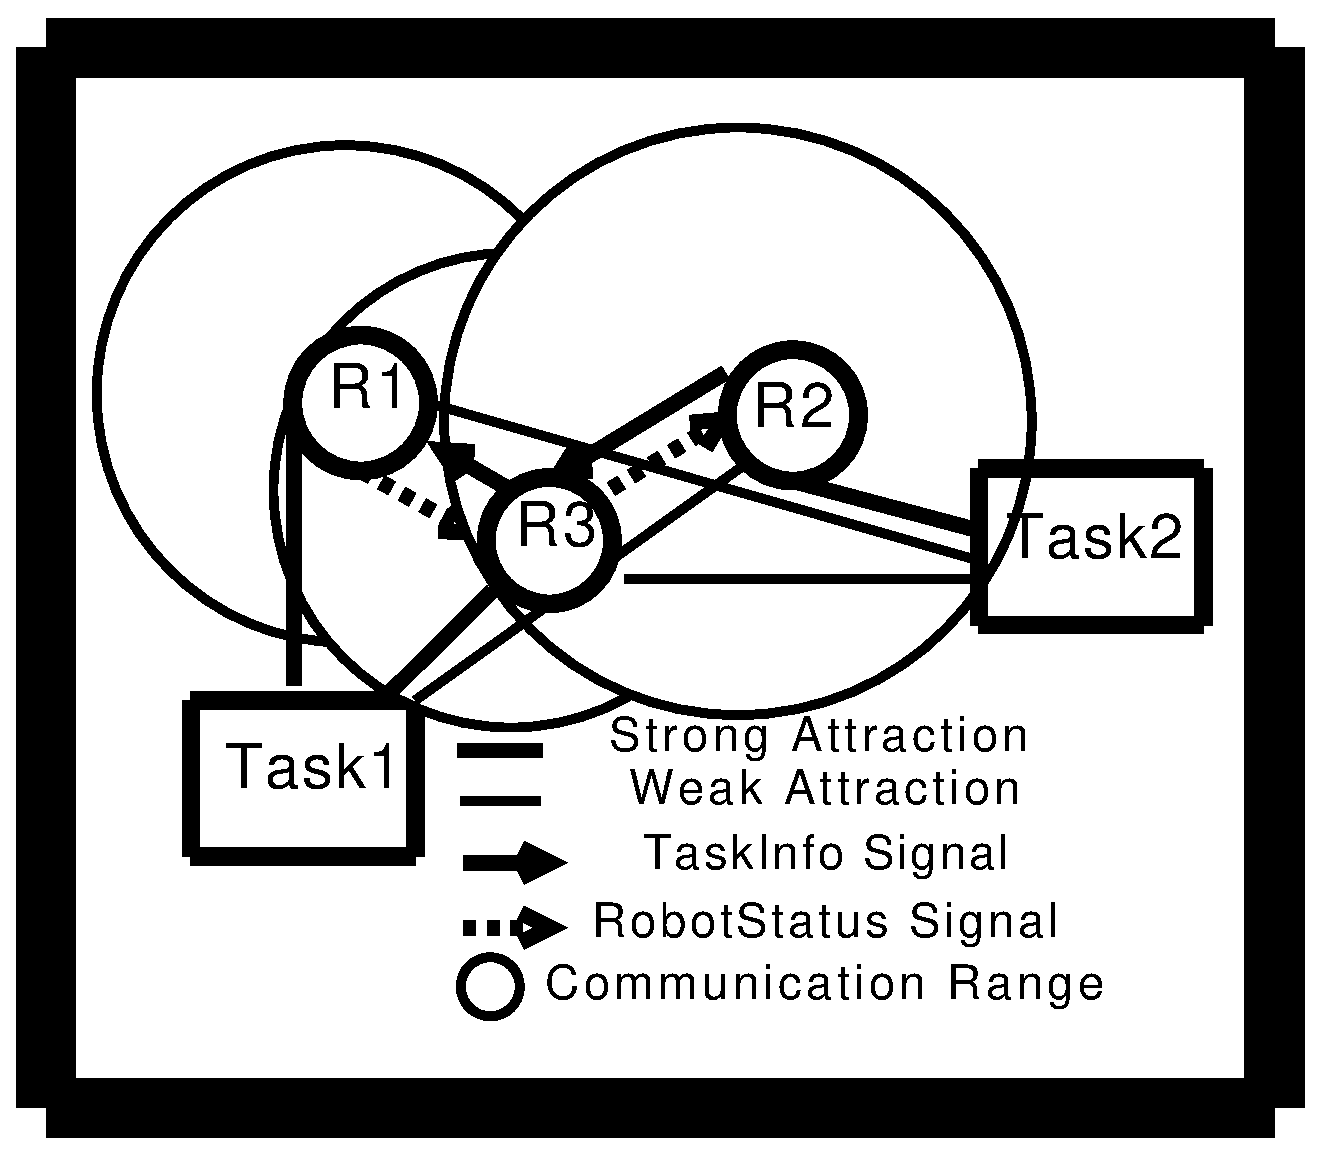
\includegraphics[height=4cm, angle=0]{../dia-files/LocalComm.eps}
% figure caption is below the figure
%\vspace*{0.20cm}
\caption{Local communication model}
\label{fig:lcm} % Give a unique label
\end{figure}
%\addtolength{\belowcaptionskip}{-15mm}
%\end{spacing}
%
%%%%%%%%%%%%%%%%%%%%%%%%%%%%%%%%%%%%%%%%%%%%%%%%%%%%%%%%%%%%%%%%%%%%%%%%%%%%%%%%
\section{Implementation}
\label{sec:impl}
\begin{figure}
\centering
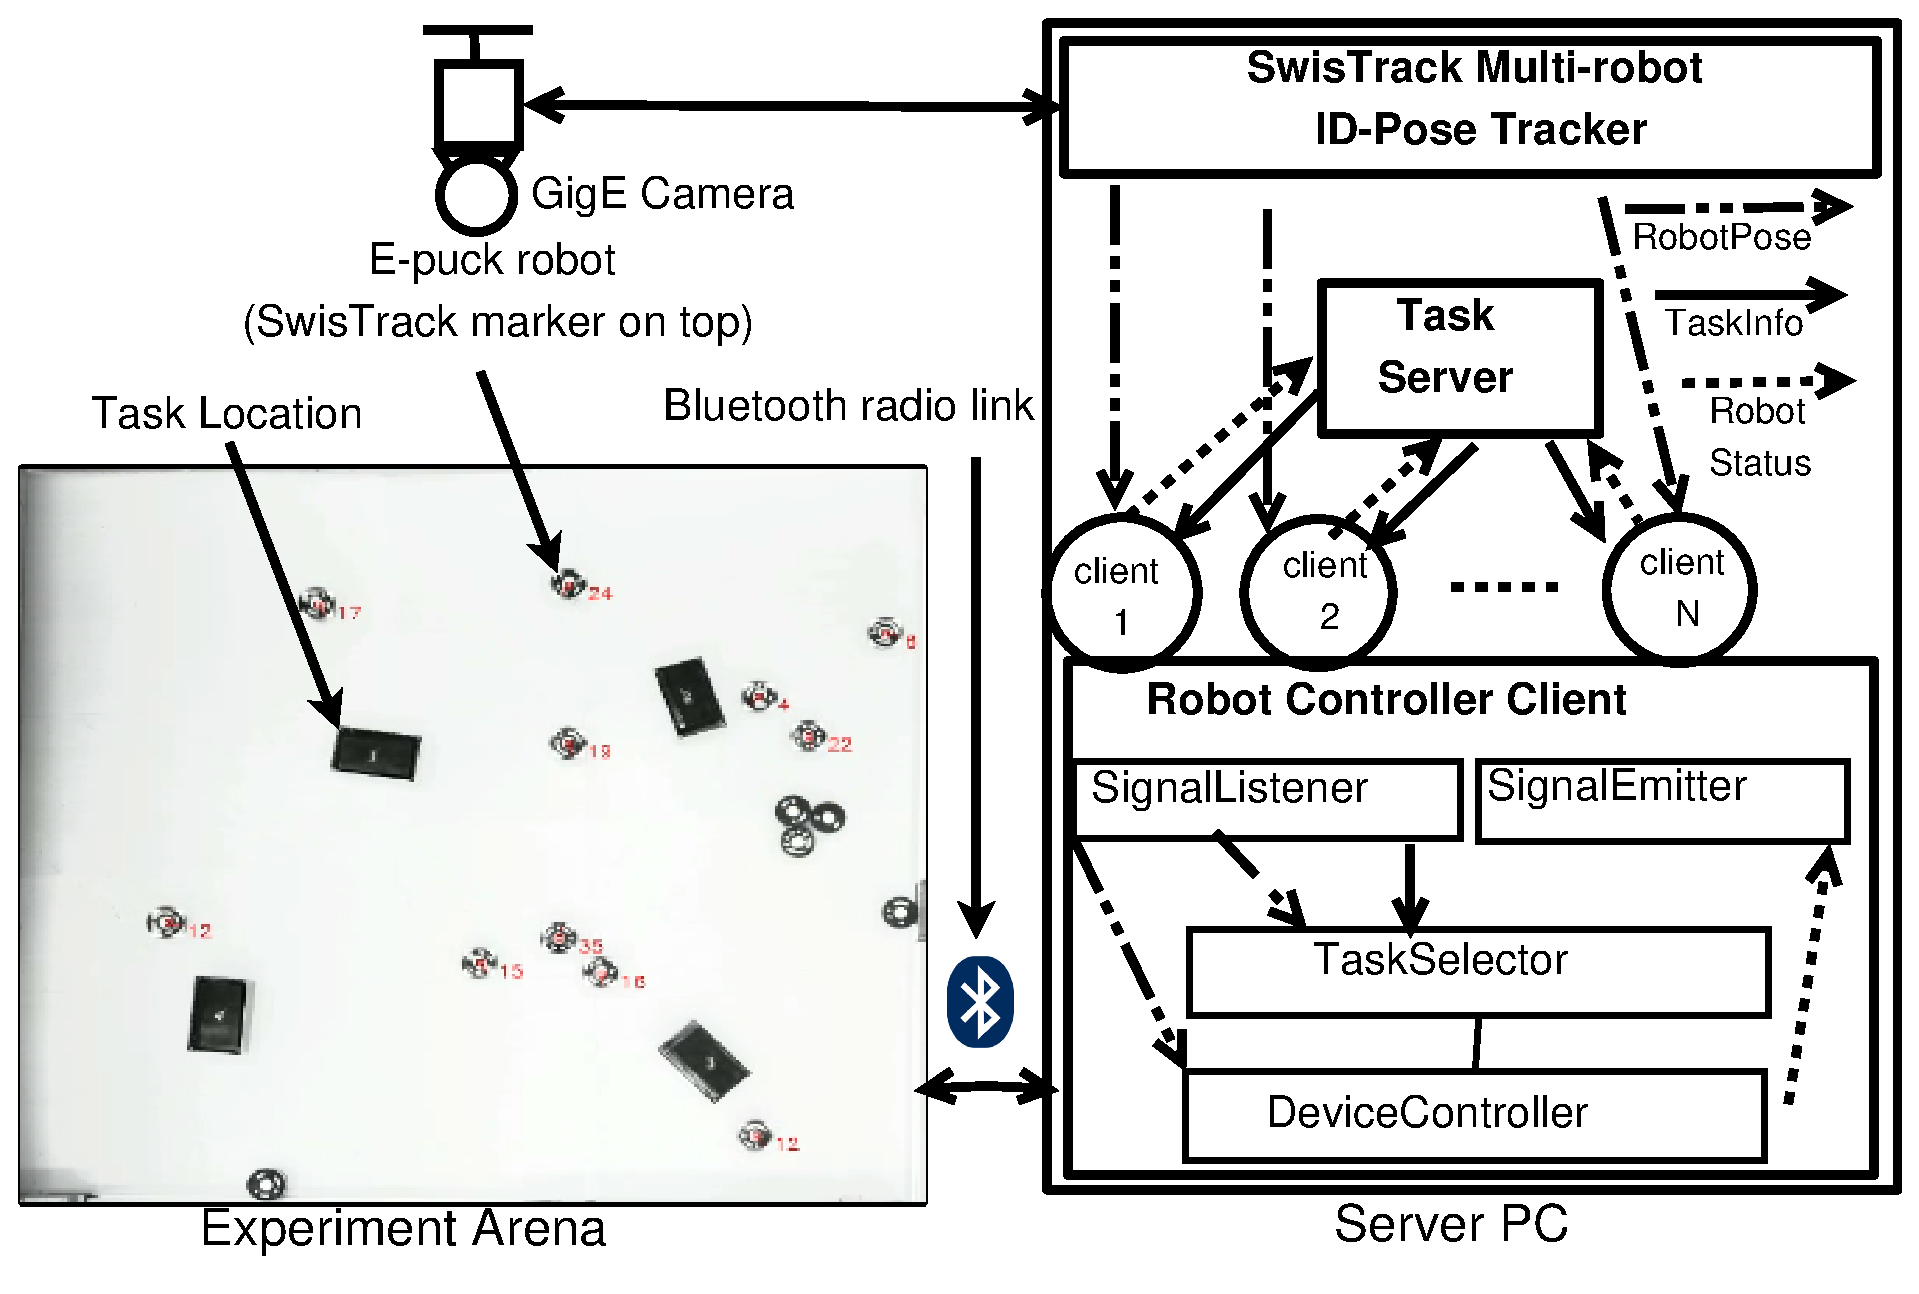
\includegraphics[height=5.5cm, angle=0]
{../dia-files/RIL-Expt-Setup1.eps}
%figure caption is below the figure
\caption{\small Hardware and software setup}
\label{fig:setup} % Give a unique label
\end{figure}
We have developed a system where up to 40 E-puck robots \cite{Epuck} can operate together according to the generic rules of the AFM. As shown in Fig. \ref{fig:setup}, our software system consists of a multi-robot tracking system, a centralized task server and robot controller clients. Here at first we have presented the design of our communication system. Then we have discussed about our specific implementation. 

%%%%%%%%%%%%%%%%%%%%%%%%%%%%%%%%%%%%%%%%%%%%%%%%%%%%%%%%%%%%%%%%%%%%%%%%%%%%%%%%%
\section{Experiment Design}
\label{sec:expt-design}
In this section, we have described the design of parameters and observables of our experiments.
These experiments are designed to validate AFM by testing the occurrence of convergent MRTA. Our experimental setup can be found in section~\ref{sec:impl}. The details of convergence is presented in section~\ref{sec:results}.
%
\begin{table}
\caption{Experimental parameters}
\label{table:params}
\begin{center}
\begin{tabular}{|l||c|}
\hline Parameter & Value\\
\hline Total number of robots ($N$) & 16\\
\hline Total number of tasks ($M$) & 4\\
\hline Experiment area ($A$) & 4 $m^2$\\
\hline Intial task urgency ($\Phi_{INIT}$) & 0.5\\
\hline Task urgency increase rate ($\Delta\phi_{INC}$) & 0.005\\
\hline Task urgency decrease rate ($\Delta\phi_{DEC}$) & 0.0025\\
\hline Intial sensitization ($K_{INIT}$) & 0.1\\
\hline Sensitization increase rate ($\Delta k_{INC}$) & 0.03\\
\hline Sensitization decrease rate ($\Delta k_{DEC}$) & 0.01\\
\hline A very small distance ($\delta$)& 0.000001\\
\hline Task info update interval ($\Delta TS_{u}$) & 5s\\
\hline Task info signal emission interval ($ \Delta TS_{e}$)& 2.5s\\
\hline Robot's task time-out interval ($\Delta RT_{to} $)& 10s\\
\hline
\end{tabular}
\end{center}
\end{table}
%%%%%%%%%%%%%%%%%%%%%%%%%%%%%%%%%%%%%%%%%%%%%%%%%%%%%%%%%%%%%%%%%%%%%%
\section{Results and Discussions}
\label{sec:results}
%%
In this section we have presented our experimental results. We ran those experiments for about 40 minutes and averaged them from three iterations.
%%% raw urgencies
\begin{figure}
\centering
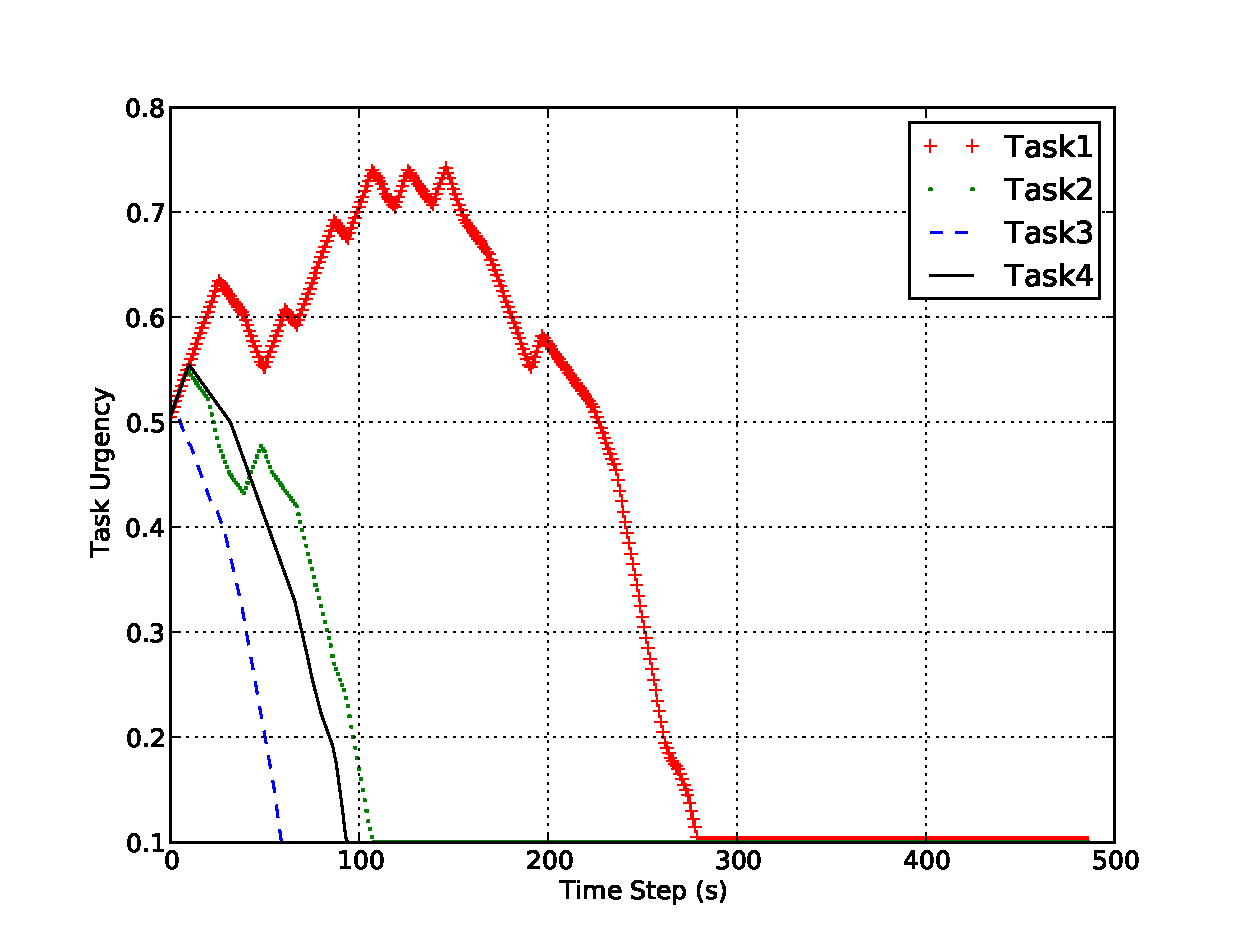
\includegraphics[height=5cm, angle=0]
{images/local-500cm/PlotUrgencyLog-2010Feb15-171017.eps}
%figure caption is below the figure
\caption{\small Task urgencies observed at TaskServer in local mode $R_{comm}$=0.5m}
\label{fig:raw-urgencies} % Give a unique label
\end{figure}
%%%
Fig. \ref{fig:raw-urgencies} shows the dynamic changes in task urgencies.
In order to describe our system's dynamic behaviour holistically we analyse the changes in task urgencies over time. Let $ \phi_{j, q}$ be the urgency of a task $j$ at $q^{th}$ step. In $(q+1)^{th}$ step, we can find the change of urgency of task $j$ :\\
\begin{equation} 
\small
\delta \phi_{j, q+1} = ( \phi_{j, q+1} - \phi_{j, q}) 
\end{equation}
So we can calculate the sum of changes in urgencies of all tasks at $(q+1)^{th}$ step:
\begin{equation} 
\small
\Delta \Phi_{j, q+1} = \sum_{j=1}^{M} \delta \phi_{j, q+1} 
\label{eqn:Delta-Phi}
\end{equation}
Fig. \ref{fig:urgency-convergence} plots this sum of changes of task urgencies by a dashed line. If we consider the absolute change over a window $w$ of time in the following equation we can describe the overall changes of our systems in both positive and negative directions.
%
\begin{equation}
\small
\Delta \Phi_{jw, q+1} = \sum_{j=0}^{w-1} \left | \Delta \Phi_{q+j} \right |
\end{equation}
%
In order to find convergence in DoL we have calculated the sum of absolute changes in task urgencies over a window of 2 consecutive steps (100s). This is plotted in solid line in Fig. \ref{fig:urgency-convergence}. Note that we scale down the time steps of this plot by aggregating the values of 10 consecutive steps (50s) of Fig. \ref{fig:raw-urgencies} into a single step value.
From Fig. \ref{fig:raw-urgencies} we can see that initially the sum of changes of task urgencies are towards negative direction. This implies that tasks are being served by a high number of robots. When the task urgencies stabilize near zero the fluctuations in urgencies become minimum. Since robots chose tasks stochastically, there will always be a small changes in task urgencies. A potential convergence point is shown in Fig. \ref{fig:urgency-convergence} by considering the persistence existence of the value of $\Delta \Phi_{jw, q+1}$ below a threshold 0.1. This convergence happens near step 23 or after 1150s from the beginning of our experiments. This implies that from this point of time and onwards, changes of our system's behaviour remains under a small threshold value.\\
%
Similar to Eq. \ref{eqn:Delta-Phi}, we can calculate the absolute sum of changes in sensitizations by all robots in the following equation.
% 
\begin{equation}
\small 
\Delta K_{j, q+1} = \sum_{j=1}^{M} \left | \Delta k_{j, q+1} \right |
\label{eqn:Delta-K}
\end{equation}
This values of $\Delta K$ are plotted in Fig. \ref{fig:sensitization-stat}. It shows that the overall rate of learning and forgetting decrease over time. It is a consequence of the gradually increased task specialization of robots.
%%%%
%%%%% Task Urgency Convergence
\begin{figure*}
\begin{minipage}[t]{0.5\linewidth}
\centering
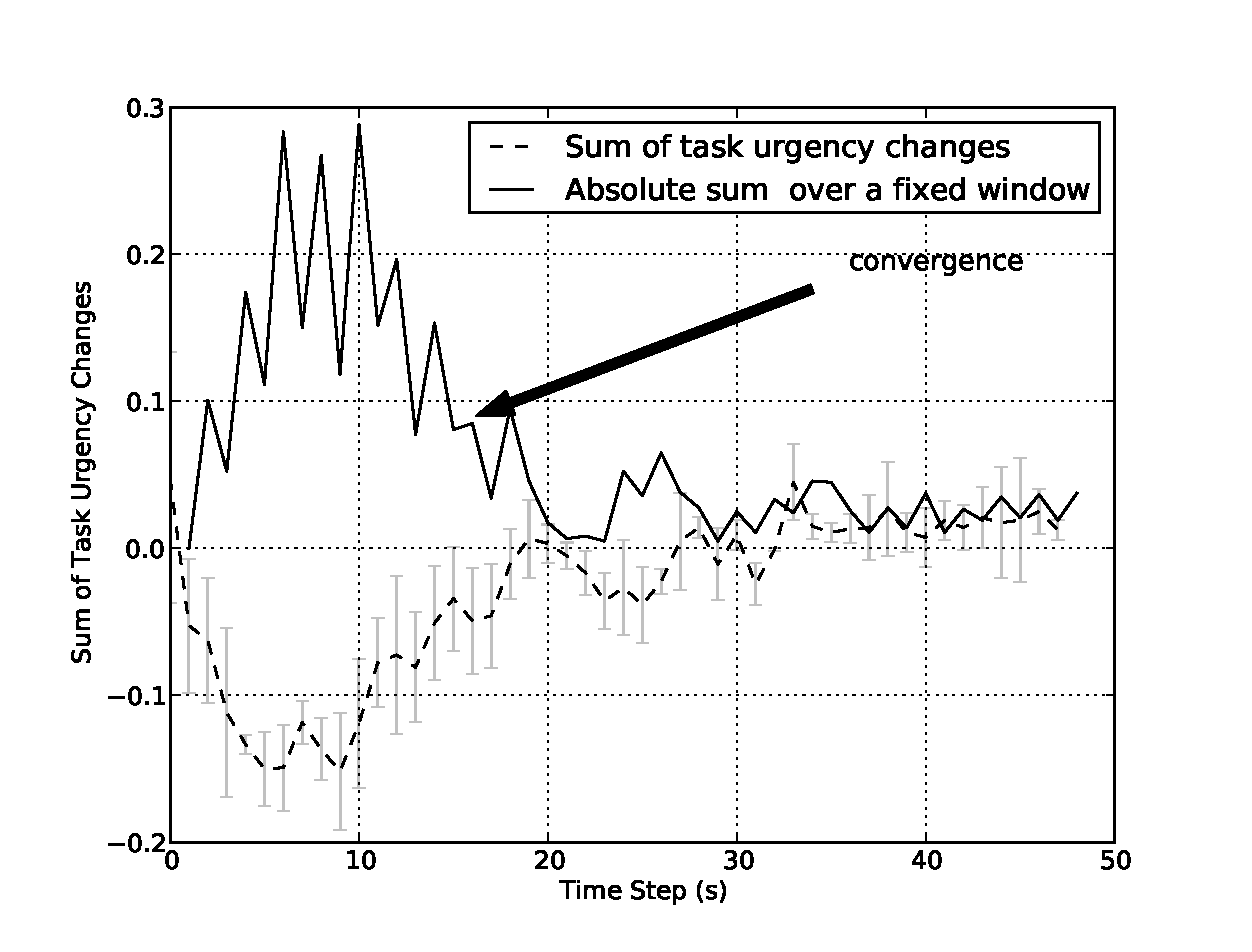
\includegraphics[height=5cm, angle=0]
{images/local-500cm/Local500cm-TaskUrgencyConvergence.eps}
%figure caption is below the figure
\caption{\small Convergence of task urgencies in local mode $R_{comm}$=0.5m}
\label{fig:l500cm-convergence} % Give a unique label
\end{minipage}
\hspace{0.5cm}
\begin{minipage}[t]{0.5\linewidth}
\centering
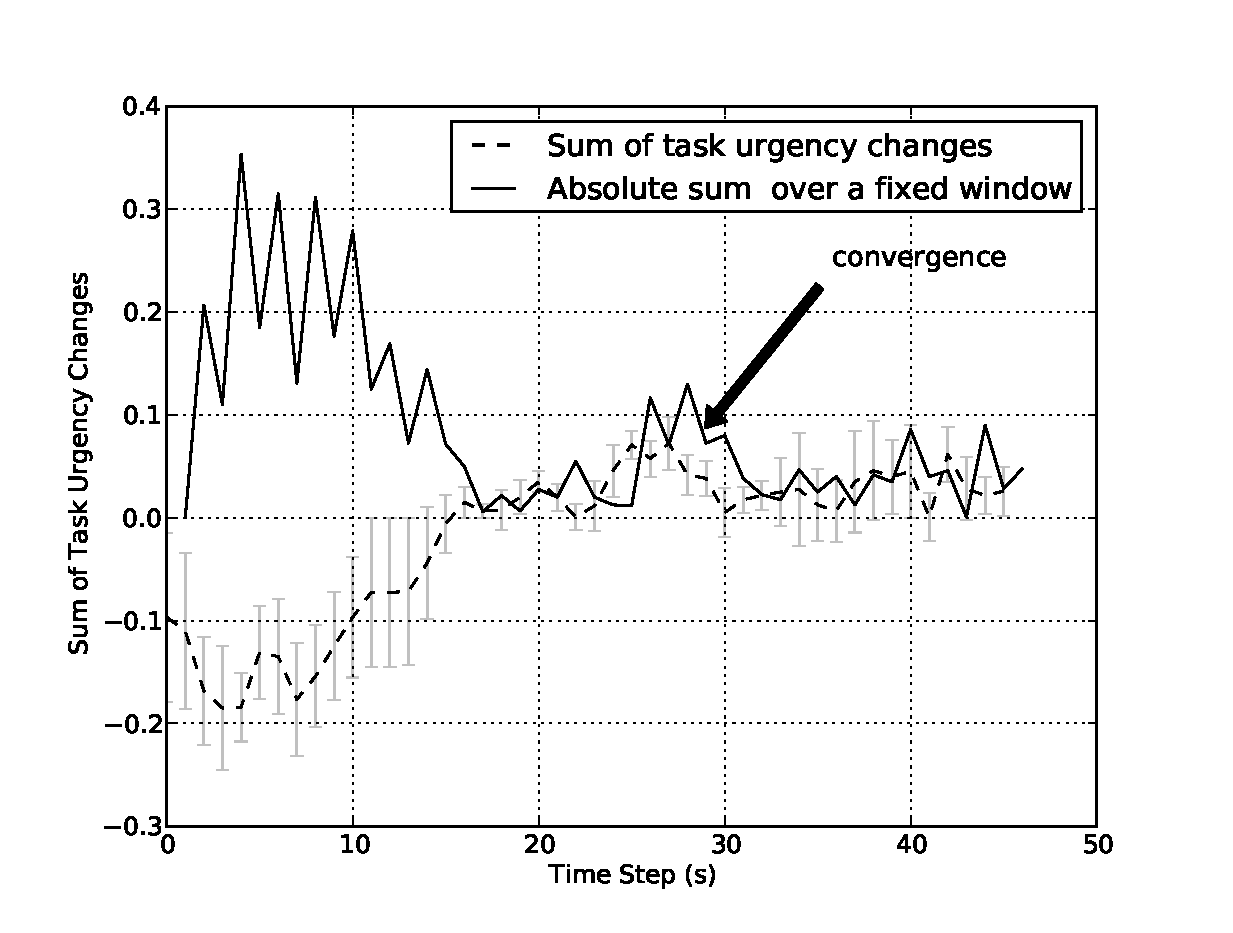
\includegraphics[height=5cm, angle=0]{images/local-1m/TaskUrgencyConvergence.eps}
\caption{\small Convergence of task urgencies in local mode $R_{comm}$=1m}
\label{fig:l1m-convergence} % Give a unique label
\end{minipage}
\end{figure*}
%%
%%% Sensitization%%%
\begin{figure*}
\begin{minipage}[t]{0.5\linewidth}
\centering
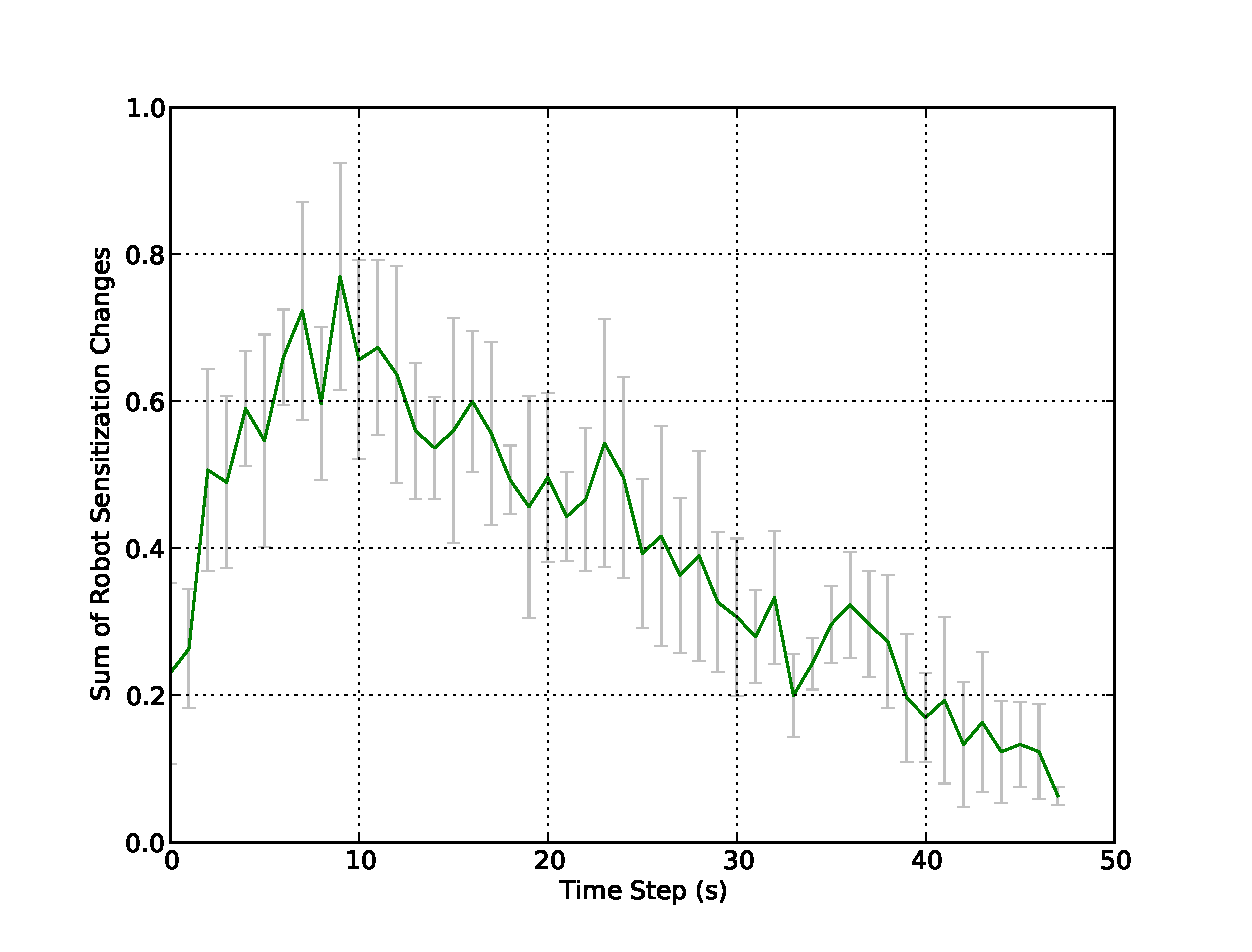
\includegraphics[height=5cm, angle=0]
{images/local-500cm/RobotSensitizationStat-Total-50steps.eps}
%figure caption is below the figure
\caption{\small Changes in sensitizations of all robots in local mode $R_{comm}$=0.5m}
\label{fig:sensitization-stat} % Give a unique label
\end{minipage}
\hspace{0.5cm}
\begin{minipage}[t]{0.5\linewidth}
\centering
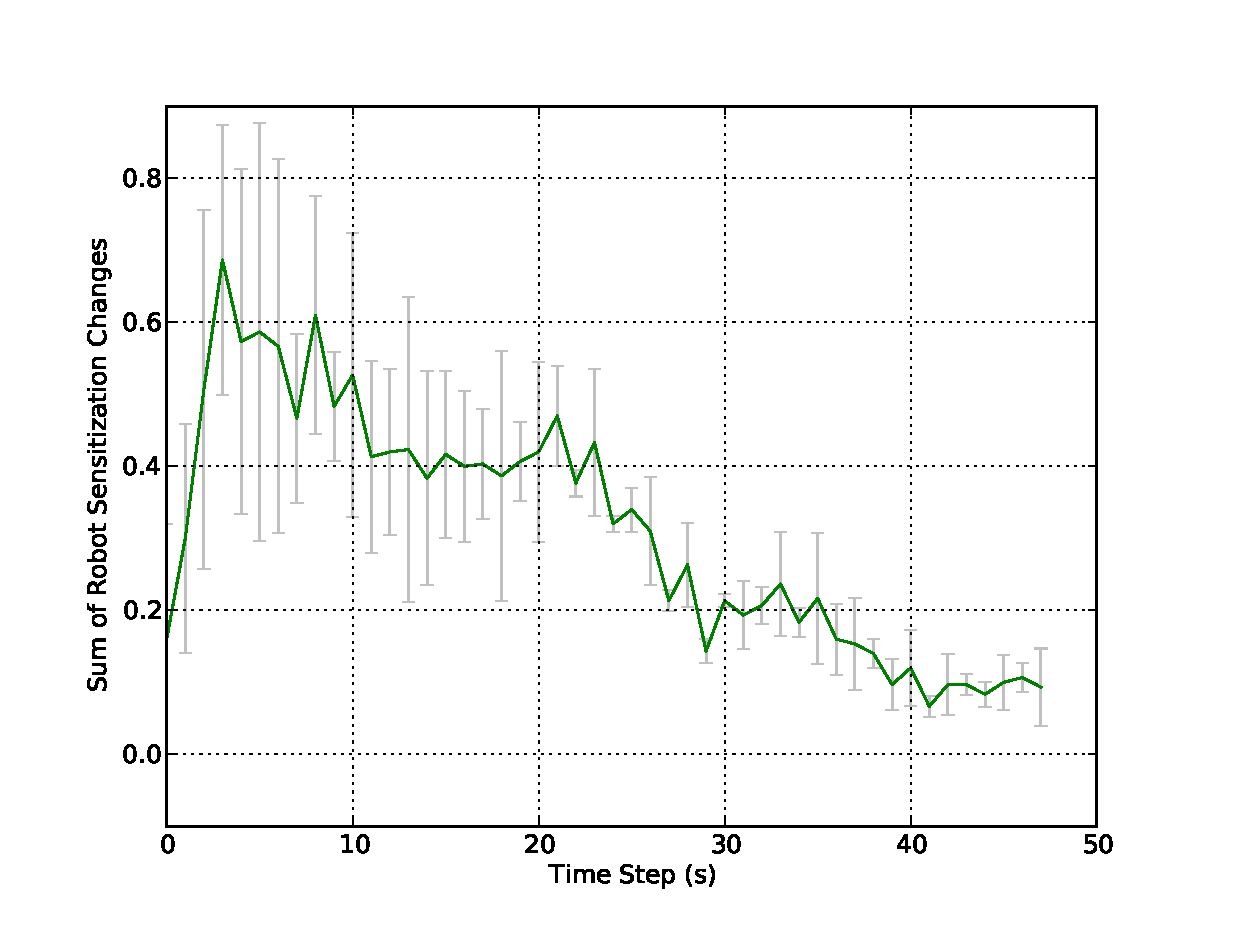
\includegraphics[height=5cm, angle=0]{images/local-1m/RobotSensitizationStat-Total-50steps.eps}
\caption{\small Changes in sensitizations of all robots in local mode $R_{comm}$=1m}
\label{fig:translation-stat} % Give a unique label
\end{minipage}
\end{figure*}
%%
%%% Translation %%%
\begin{figure*}
\begin{minipage}[t]{0.5\linewidth}
\centering
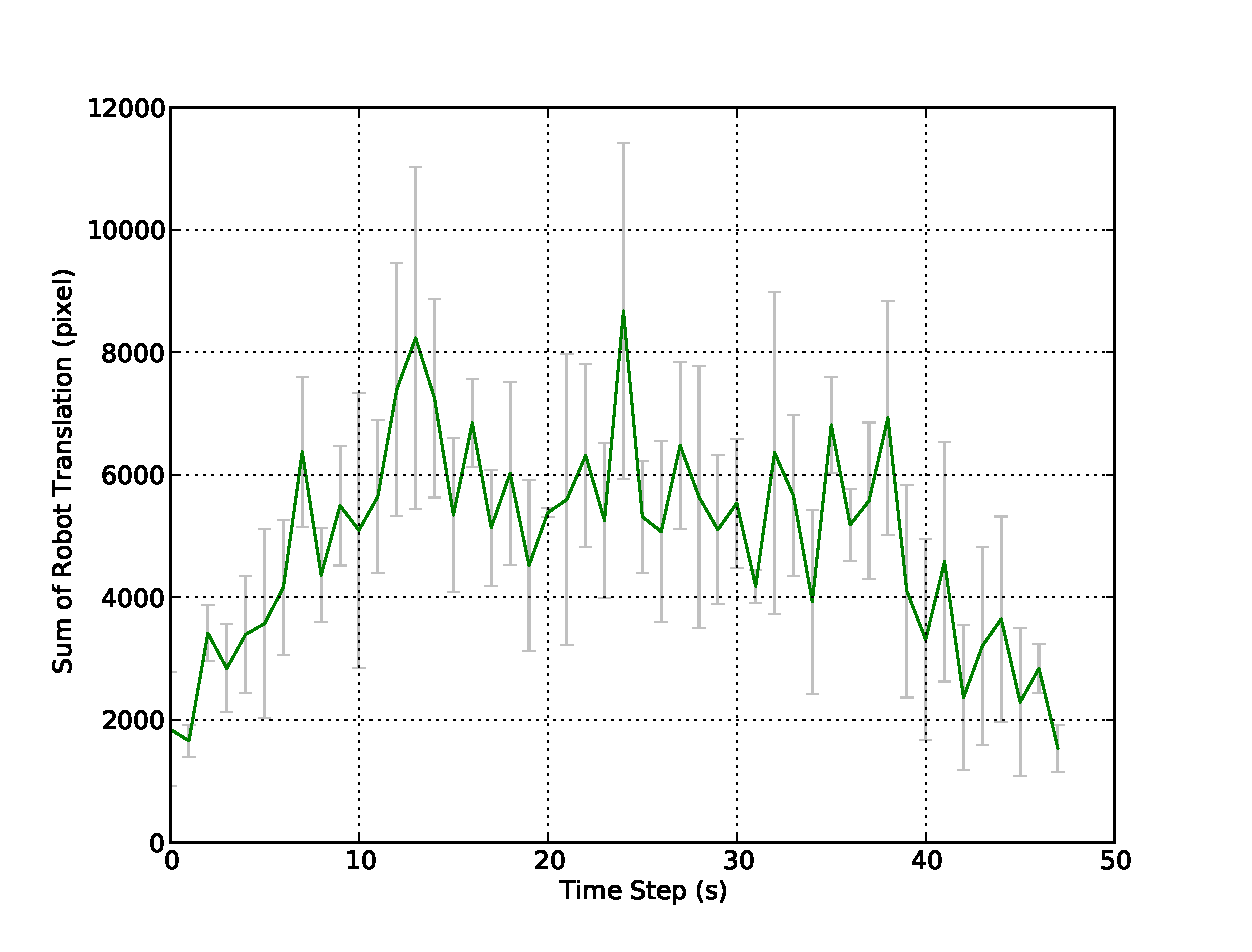
\includegraphics[height=5cm, angle=0]
{images/local-500cm/DeltaTranslationStat.eps}
%figure caption is below the figure
\caption{\small Sum of translations of all robots in local mode $R_{comm}$=1m }
\label{fig:sensitization-stat} % Give a unique label
\end{minipage}
\hspace{0.5cm}
\begin{minipage}[t]{0.5\linewidth}
\centering
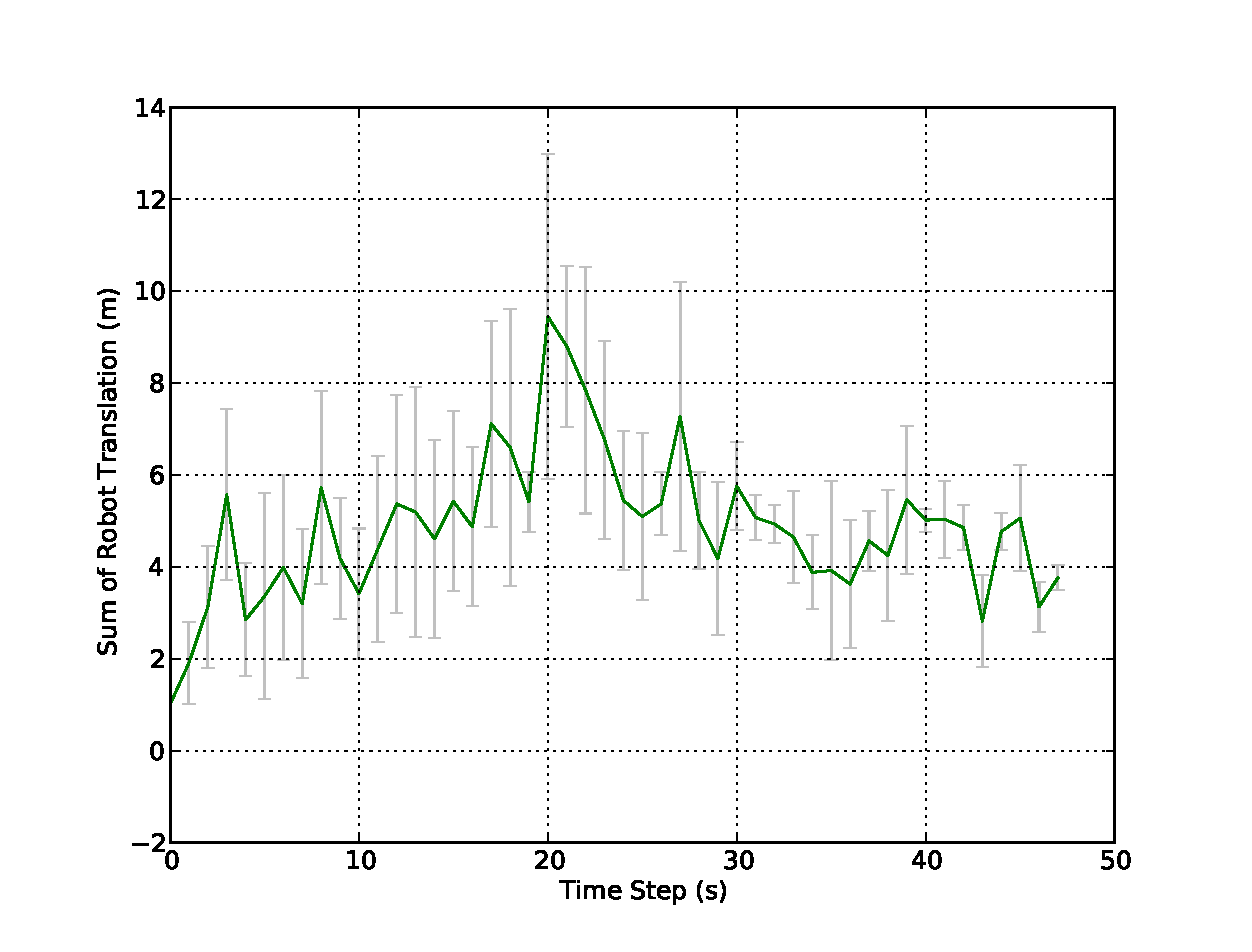
\includegraphics[height=5cm, angle=0]{images/local-1m/DeltaTranslationStat.eps}
\caption{\small Sum of translations of all robots in local mode $R_{comm}$=1m }
\label{fig:translation-stat} % Give a unique label
\end{minipage}
\end{figure*}

We have aggregated the changes in translation motion of all robots over time. Let $u_{i,q}$ and $u_{i,q+1}$ be the translations of a robot $i$ in two consecutive steps. If the difference between these two translations be $\delta u_{i}$, we can find the sum of changes of translations of all robots in $(q+1)^{th}$ step using the following equation.
\begin{equation}
\small 
\Delta U_{q+1} = \sum_{i=1}^{N} \delta u_{i, q+1} 
\label{eqn:Delta-Tr}
\end{equation}
This is plotted in Fig. \ref{fig:translation-stat}. In this plot we can see that robot translations also vary over varying task requirements of tasks. But it fails to show a consistence behaviour like previous plots.\\
%
%%% Communication load %%%
\begin{figure*}
\begin{minipage}[t]{0.5\linewidth}
\centering
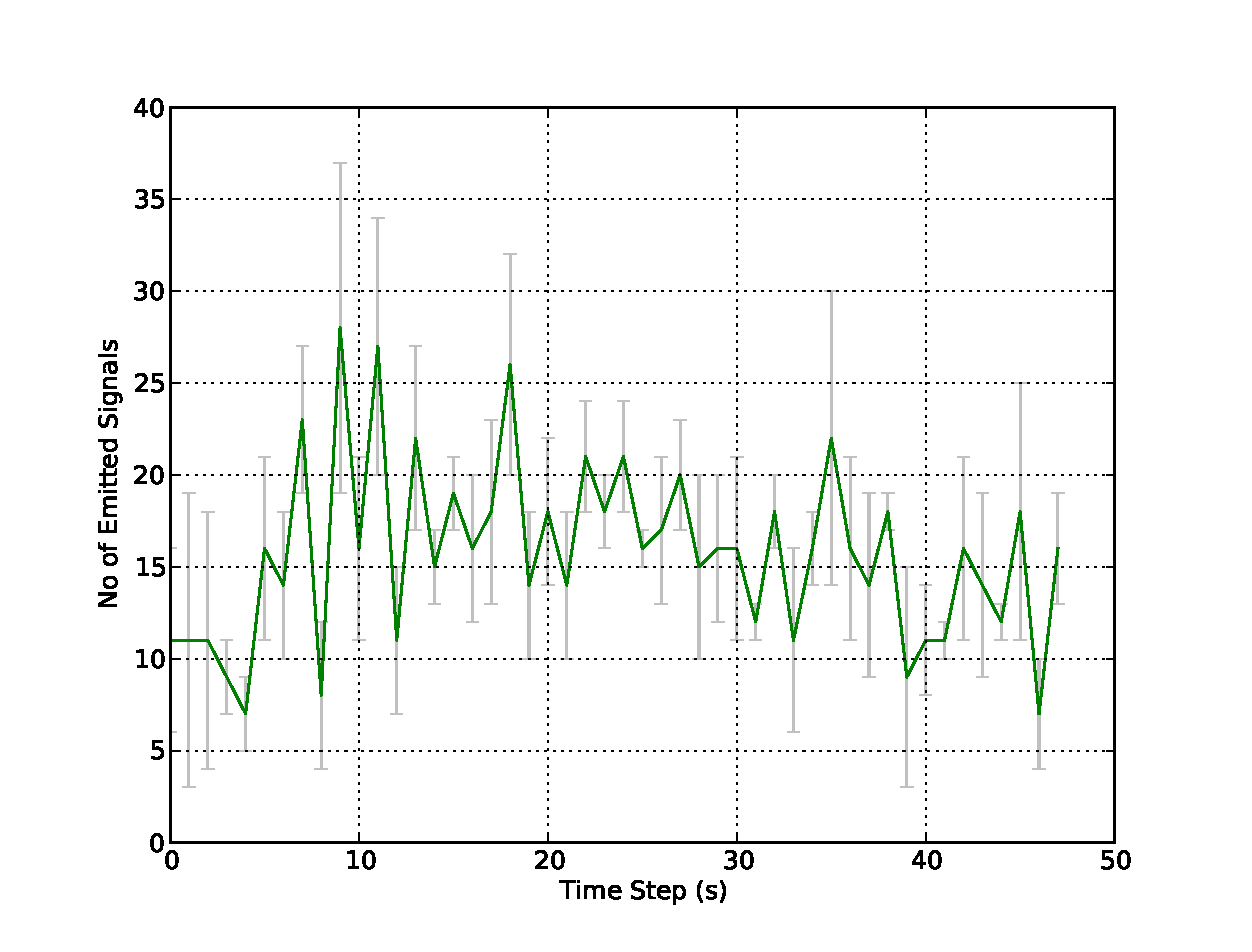
\includegraphics[height=5cm, angle=0]
{images/local-500cm/Local-500cm-SignalingFreqStat.eps}
\caption{\small Local peers' frequency of task information signalling in local mode $R_{comm}$=0.5m}
\label{fig:signal-frequency-stat} % Give a unique label
\end{minipage}
\hspace{0.5cm}
\begin{minipage}[t]{0.5\linewidth}
\centering
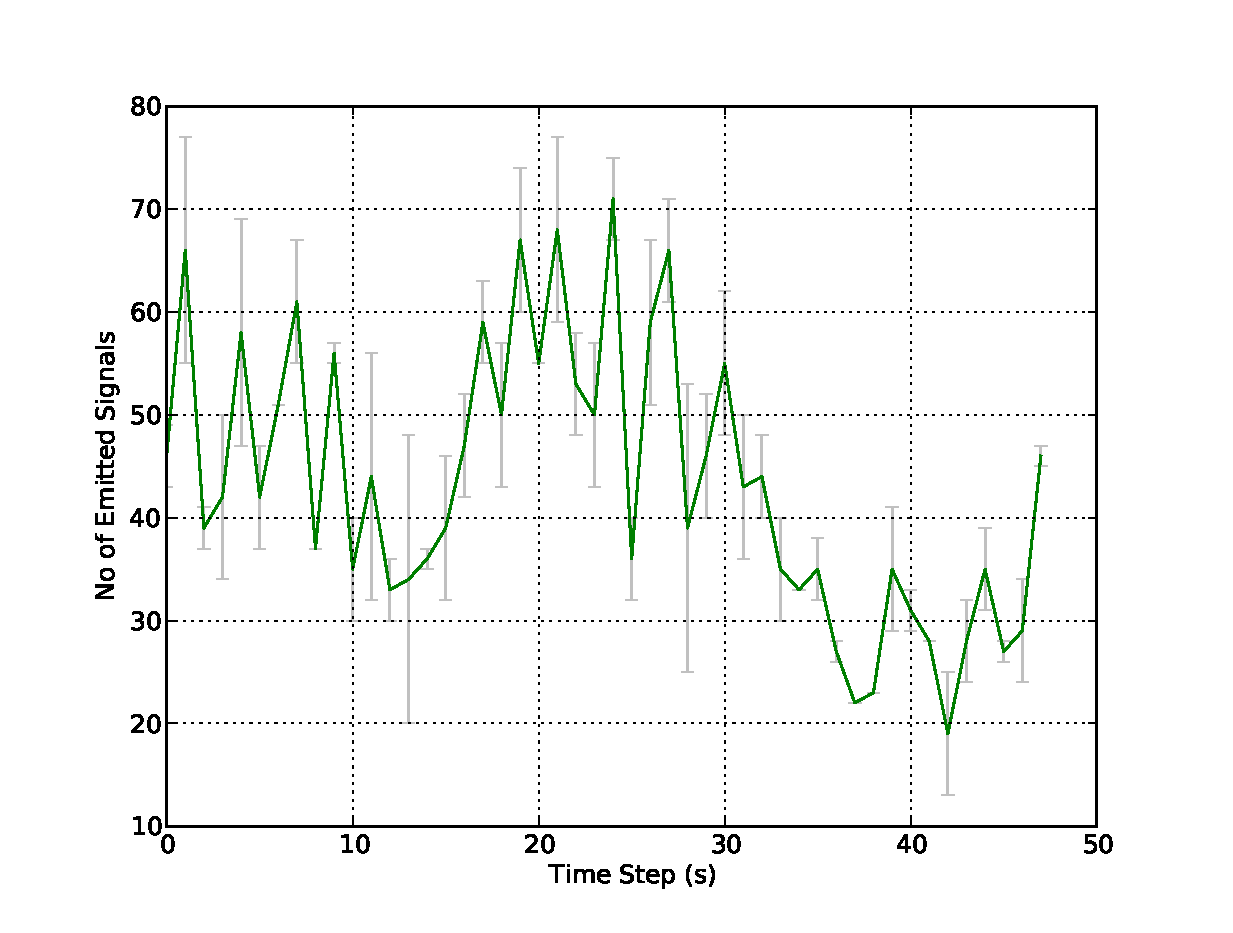
\includegraphics[height=5cm, angle=0]{images/local-1m/Local-1m-SignalingFreqStat.eps}
\caption{\small Local peers' frequency of task information signalling in local mode $R_{comm}$=1m}
\label{fig:translation-stat} % Give a unique label
\end{minipage}
\end{figure*}
%
Fig. \ref{fig:signal-frequency-stat} presents the frequency of signalling task information by TaskServer. Since the duration of each time step is 50s long and TaskServer emits signal in every 2.5s, there should be 20 signals in each step. The insignificant variation in frequency shows us the stable behaviour of D-Bus daemon over time.
%
%%%% Single- robot sensitization and translation
\begin{figure*}
\begin{minipage}[t]{0.5\linewidth}
\centering
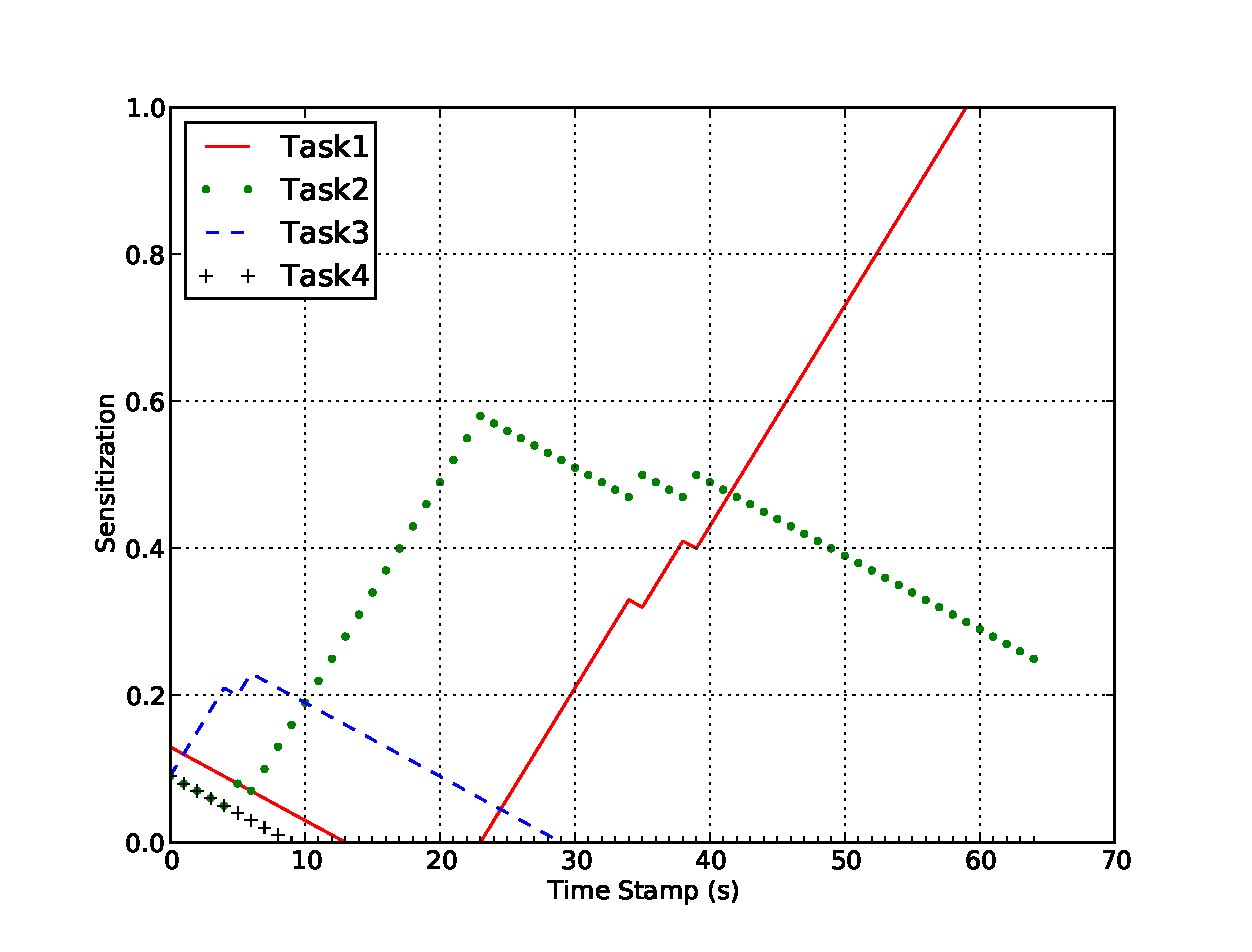
\includegraphics[height=5cm, angle=0]{images/local-500cm/PlotRobot12-Sensitizations-2010Feb16-150432.eps}
\caption{\small Task specialization of Robot12 in local mode $R_{comm}$=0.5m}
\label{fig:single-robot-sensitizations} % Give a unique label
\end{minipage} 
%%%
\begin{minipage}[t]{0.5\linewidth}
\centering
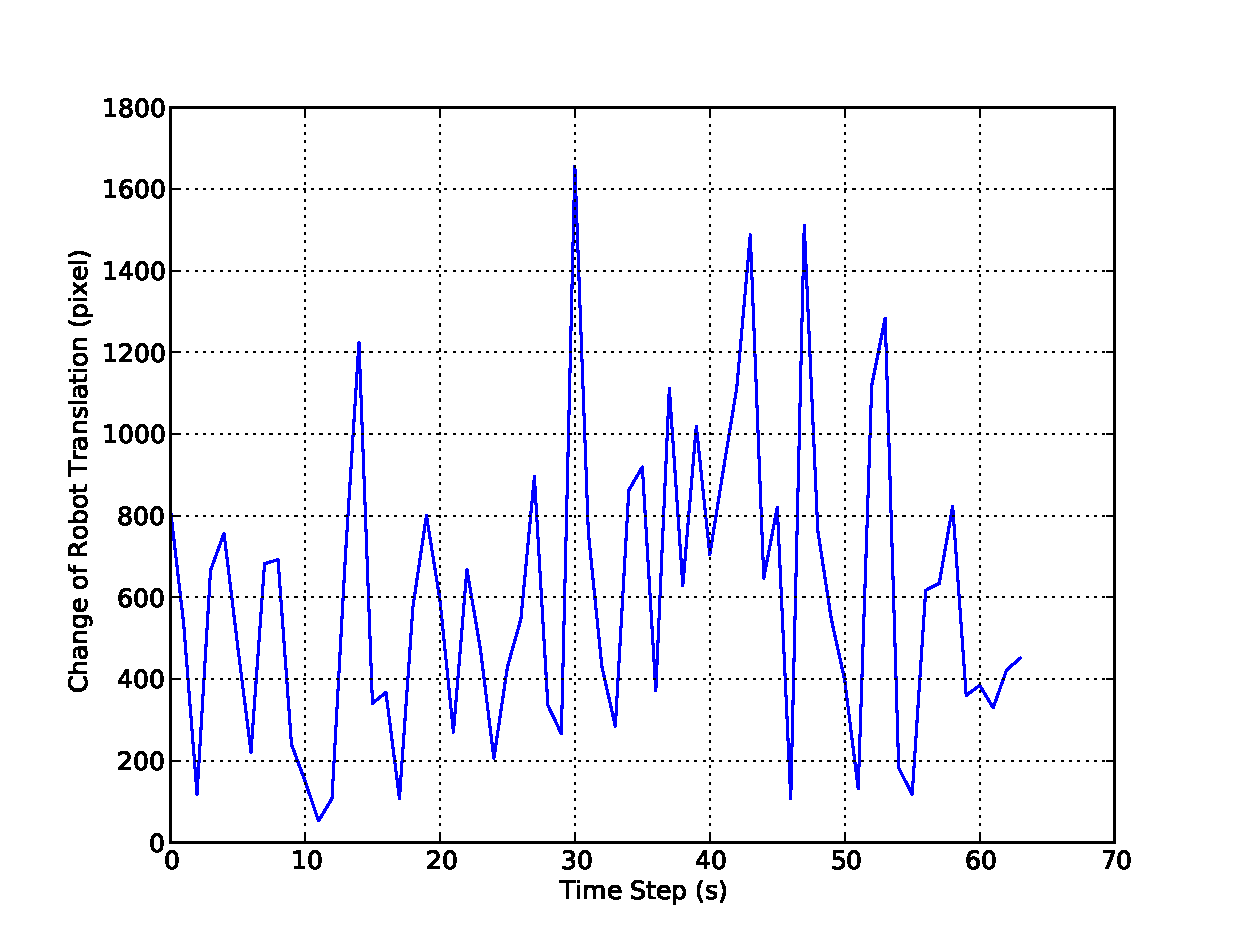
\includegraphics[height=5cm, angle=0]{images/local-500cm/DeltaRobot12-PoseAtTS-2010Feb16-150432.eps}
\caption{\small Changes in translation of Robot12 in local mode $R_{comm}$=0.5m}
\label{fig:single-robot-translation} % Give a unique label
\end{minipage}
\end{figure*}
%%%%
%%%% Single- number of peers
\begin{figure*}
\begin{minipage}[t]{0.5\linewidth}
\centering
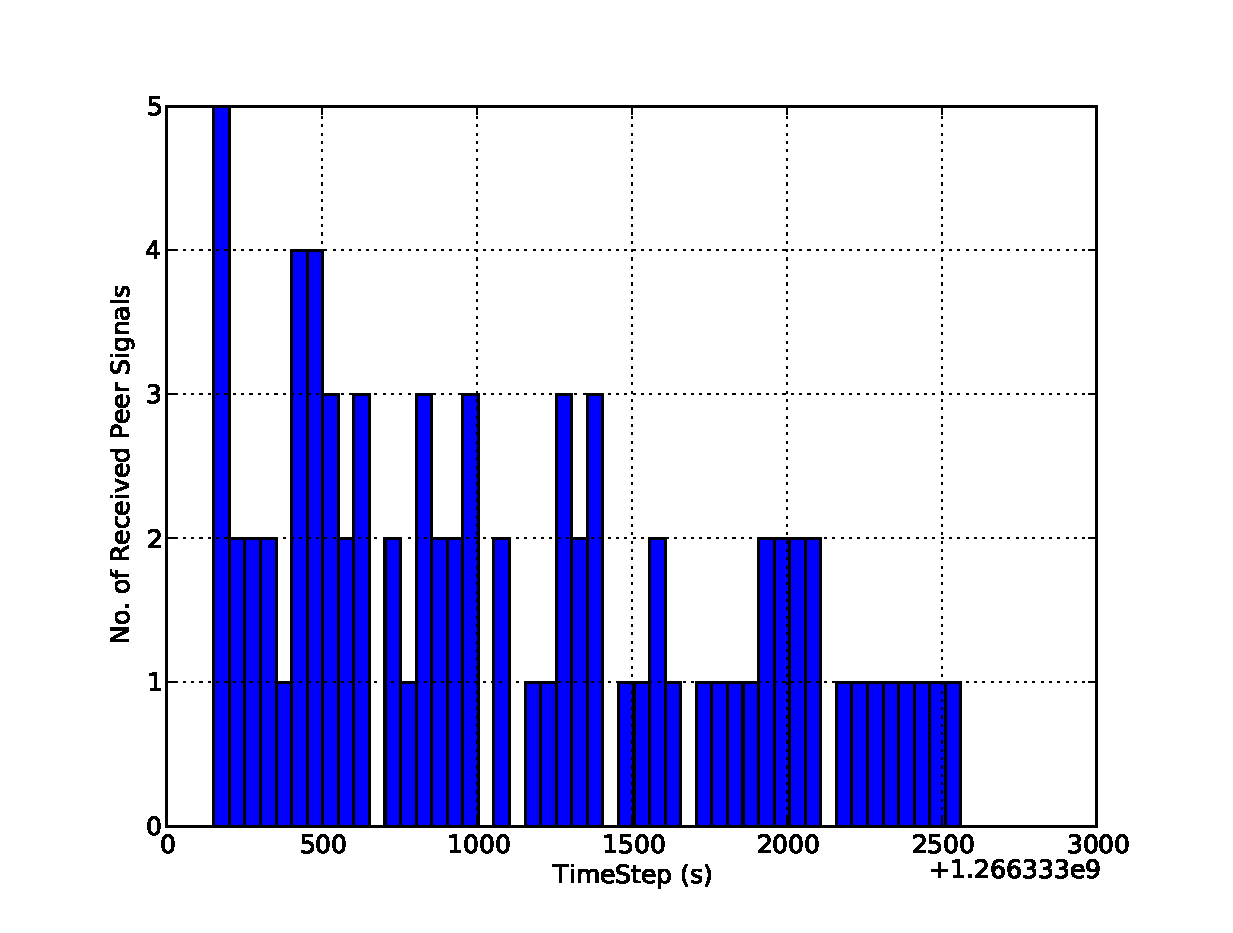
\includegraphics[height=5cm, angle=0]{images/local-500cm/Robot12-16feb-1-LocalSignals.eps}
\caption{\small Number of peer signals caught by Robot12 in local mode $R_{comm}$=0.5m}
\label{fig:single-robot-sensitizations} % Give a unique label
\end{minipage} 
%%%
\begin{minipage}[t]{0.5\linewidth}
\centering
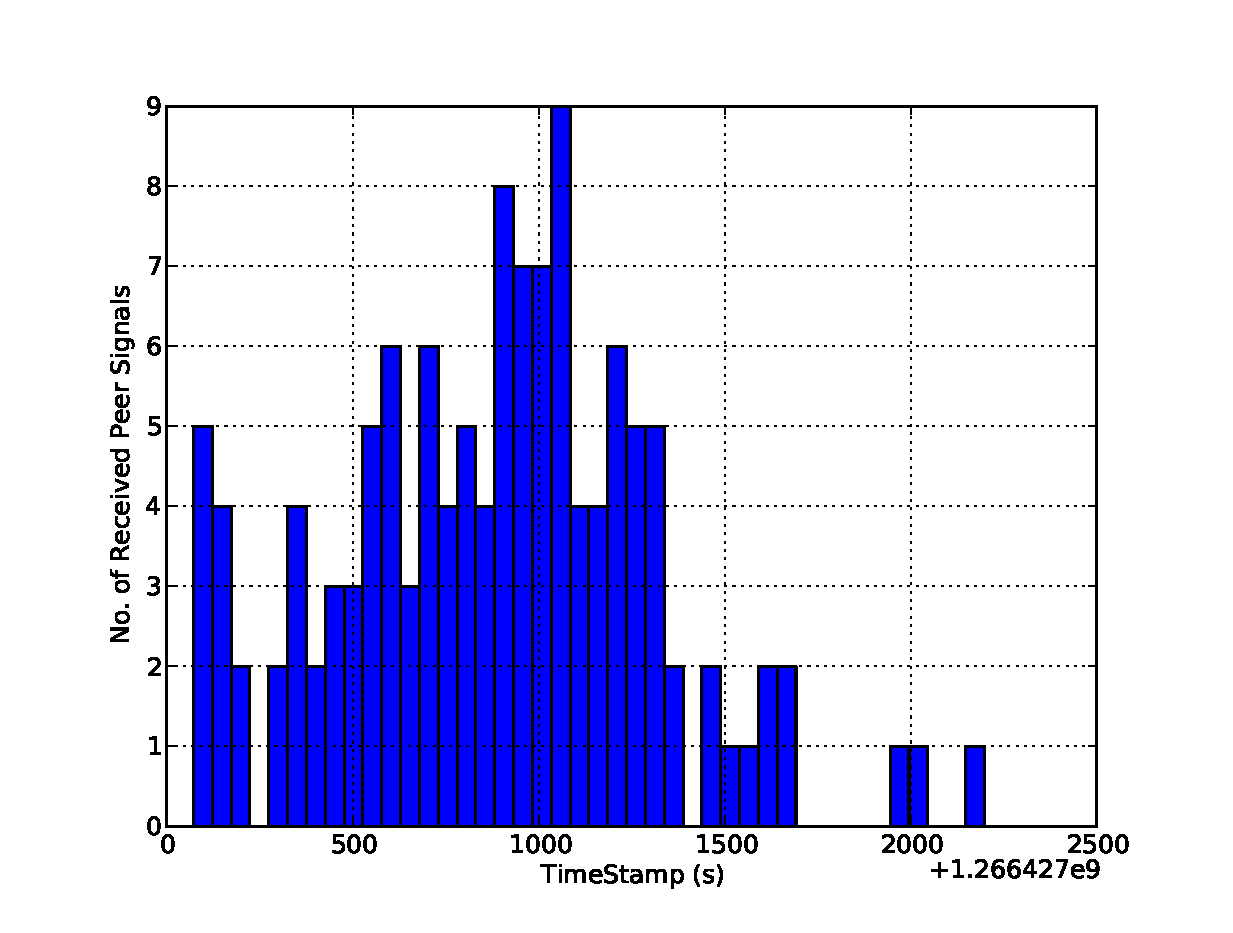
\includegraphics[height=5cm, angle=0]{images/local-1m/Robot12-17feb-3-LocalSignals.eps}
\caption{\small  Number of peer signals caught by Robot12 in local mode $R_{comm}$=1m}
\label{fig:single-robot-translation} % Give a unique label
\end{minipage}
\end{figure*}


As an example of task specialization of a robot we plotted sensitization of Robot9 in Fig. \ref{fig:single-robot-sensitizations}. It shows that this robot has specialized in Task1. The continuous learning happens from step 12 to step 42 where it has learned this task completely and forgot rest of the tasks. This behaviour is found common in all robots with varying level of sensitizations. Hence we get the linear decrease of $\Delta K$ in Fig. \ref{fig:sensitization-stat}. However, the changes in motion of this robot plotted in Fig. \ref{fig:single-robot-translation} is not stable due to the fact that robots frequently avoid dynamic obstacles and select random-walking.
%
%%%%%%%%%%%%%%%%%%%%%%%%%%%%%%%%%%%%%%%%%%%%%%%%%%%%%%%%%%%%%%%%%%%%%%%%%%%%%%%%
\section{CONCLUSIONS AND FUTURE WORKS}
\label{sec:conc}
%%%%%%%%%%%%%%%%%%%%%%%%%%%%%%%%%%%%%%%%%%%%%%%%%%%%%%%%%%%%%%%%%%%%%%%%%%%%%%%%
\begin{thebibliography}{99}
\bibitem{Bonabeau+1999}
Bonabeau, E., Dorigo, M. and Theraulaz, G.:
Swarm intelligence: from natural to artificial systems.
Oxford University Press (1999)
\bibitem{Labella}
Labella, T. H.; Dorigo, M. and Deneubourg, J. Division of labor in a group of robots inspired by ants' foraging behavior ACM Trans. Auton. Adapt. Syst., ACM, 2006, 1, 4-25
\bibitem{Elsa}
Arcaute, E.; Christensen, K.; Sendova-Franks, A.; Dahl, T.; Espinosa, A. and Jensen, H. J. : 
Division of labour in ant colonies in terms of attractive fields. 
Ecological Complexity, Elsevier (2008)
\bibitem{SwisTrack}
Lochmatter T., Roduit P., Cianci C., Correll N., Jacot J., and Martinoli A.: 
SwisTrack - A Flexible Open Source Tracking Software for Multi-Agent Systems. 
In Proceedings of the IEEE/RSJ 2008 International Conference on Intelligent Robots and Systems (IROS 2008), 4004-4010, IEEE (2008)
\bibitem{Epuck}
Cianci, C.; Raemy, X.; Pugh, J. and Martinoli, A. Communication in a swarm of miniature robots: The e-puck as an educational tool for swarm robotics Swarm robotics: second SAB 2006 international workshop, Rome, Italy, September 30-October 1, 2006: revised selected papers, 2007, 103
\bibitem{Sarker}
M. O. F. Sarker and T. S. Dahl, Robotic Validation of an Inter-disciplinary Generic
Model of Self-regulated Division of Labour in Social Systems, ANTS 2010, 7th International Conference on Swarm Intelligence (submitted, available upon request).
\bibitem{Balch}
Balch, T. and Arkin, R. Communication in reactive multiagent robotic systems Autonomous Robots, Springer, 1994, 1, 27-52
\bibitem{Gerkey}
Gerkey, B. and Mataric, M. Principled communication for dynamic multi-robot task allocation Experimental Robotics VII, 2001, 353-362
\bibitem{Rutishauser}
Rutishauser, S.; Correll, N. and Martinoli, A. Collaborative coverage using a swarm of networked miniature robots Robotics and Autonomous Systems, Elsevier, 2009, 57, 517-525
\bibitem{Krieger}
Krieger, M. and Billeter, J. The call of duty: Self-organised task allocation in a population of up to twelve mobile robots Robotics and Autonomous Systems, Citeseer, 2000, 30, 65-84
\bibitem{Agassounon}
Agassounon, W. and Martinoli, A. Efficiency and robustness of threshold-based distributed allocation algorithms in multi-agent systems Proceedings of the first international joint conference on Autonomous agents and multiagent systems: part 3, 2002, 1090-1097
\bibitem{Mataric}
Mataric, M. Using communication to reduce locality in distributed multiagent learning Journal of experimental and theoretical artificial intelligence, 1998, 10, 357-369
\bibitem{RobotTeam}
Balch, T. and Parker, L. Robot Teams: From Diversity to Polymorphism, AK Peters, Ltd., 2002

%\bibitem{c1}
%J.G.F. Francis, The QR Transformation I, {\it Comput. J.}, vol. 4, 1961, pp 265-271.
%
%\bibitem{c2}
%H. Kwakernaak and R. Sivan, {\it Modern Signals and Systems}, Prentice Hall, Englewood Cliffs, NJ; 1991.
%
%\bibitem{c3}
%D. Boley and R. Maier, "A Parallel QR Algorithm for the Non-Symmetric Eigenvalue Algorithm", {\it in Third SIAM Conference on Applied Linear Algebra}, Madison, WI, 1988, pp. A20.

\end{thebibliography}

\end{document}
